\documentclass[simplex.tex]{subfiles}
% NO NEED TO INPUT PREAMBLES HERE
% packages are inherited; you can compile this on its own

\onlyinsubfile{
\title{NeuroData SIMPLEX Report: Subfile}
}

\begin{document}
\onlyinsubfile{
\maketitle
\thispagestyle{empty}

The following report documents the progress made by the labs of Randal~Burns and Joshua~T.~Vogelstein at Johns Hopkins University towards goals set by the DARPA SIMPLEX grant.

%%%% Table of Contents
\tableofcontents

%%%% Publications
\bibliographystyle{IEEEtran}
\begin{spacing}{0.5}
\section*{Publications, Presentations, and Talks}
%\vspace{-20pt}
\nocite{*}
{\footnotesize	\bibliography{simplex}}
\end{spacing}
%%%% End Publications
}

\subsection{Multiscale Network Test}


%To guarantee validity and consistency of MGC applied to testing in
%network, we should find independent and identically distributed (i.i.d.)
%configuration of each vertex in a graph (network), of which metric well
%reflects the distance between vertices. We demonstrated that Euclidean
%distance of raw adjacency matrix does not satisfy i.i.d assumption
%generally; while diffusion maps at every time step are i.i.d under
%certain latent function, which is supported by Aldous-Hoover
%representation theorem and de Finette’s theorem. On the other hand,
%under these theorem, graph is empty or dense. Fortunately, we have found
%that exchangeable graph can be generated more generally, even containing
%sparse graphs. We generate a simple simulation to check whether MGC
%works or not. Thus we are going to test independence between diffusion
%maps at each time point $t$ and nodal attribute $X$. 
%
%For simulation, Stochastic Block Model (SBM) and additive and
%multiplicative network model have been explored which also exhibit
%non-linear dependence properties. What MGC does in this case is to test
%distance matrix of diffusion maps and nodal attributes, considering
%$(k,l)$  nearest neighbors in each.
%
%\begin{figure}[h!]
%\begin{cframed}
%\centering
%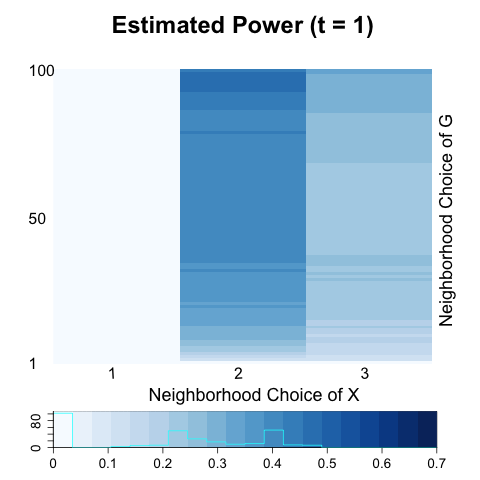
\includegraphics[width=0.45\textwidth]{../../figs/msnt1.png}
%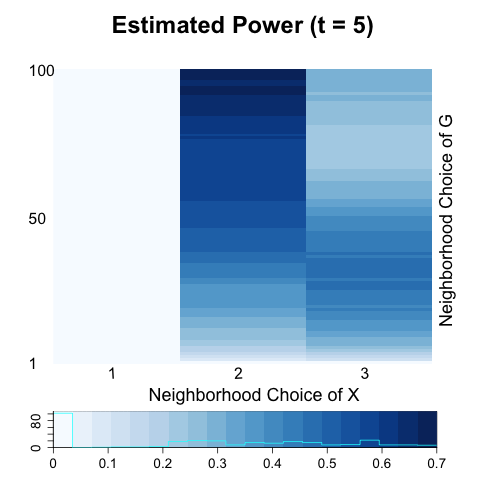
\includegraphics[width=0.45\textwidth]{../../figs/msnt2.png}
%\caption{
%The above figures illustrate power maps of
%three-block stochastic block model in terms of - nearest neighbor choice
%in terms of network diffusion maps and $k$-nearest neighbor choice in
%terms of nodal attributes. You can also notice that diffusion time
%matters in testing. 
%}
%\label{fig:msnt}
%\end{cframed}
%\end{figure}
%
%Thus if there exists
%local dependency structures or nonlinearity, the optimal neighborhood
%choice of $(k,l)$ would not count every node in network in compute
%distance correlation matrix. We also demonstrated that testing power of MGC
%applied to diffusion maps is higher in SBM and also degree-corrected
%SBM, compared to dCov, Heller-Heller-Gorfine, and latent factor network
%test proposed by Fosdick and Hoff (2015).

\end{document}
